% Created by tikzDevice version 0.8.1 on 2015-05-30 12:37:59
% !TEX encoding = UTF-8 Unicode
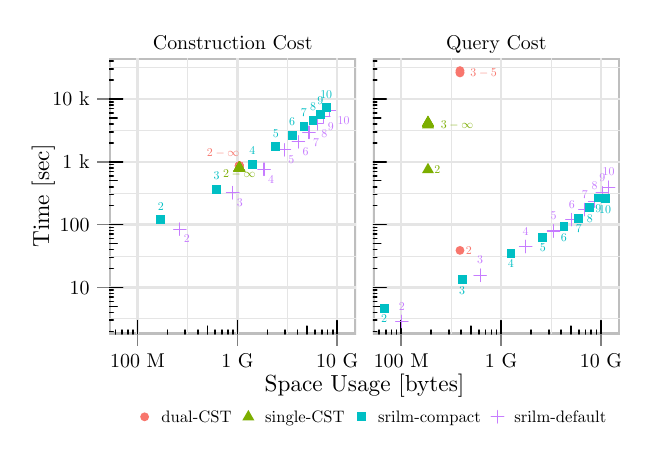
\begin{tikzpicture}[x=1pt,y=1pt]
\definecolor{fillColor}{RGB}{255,255,255}
\path[use as bounding box,fill=fillColor,fill opacity=0.00] (0,0) rectangle (216.81,144.54);
\begin{scope}
\path[clip] (  0.00,  0.00) rectangle (216.81,144.54);
\definecolor{fillColor}{RGB}{255,255,255}

\path[fill=fillColor] (  0.00,  0.00) rectangle (216.81,144.54);
\end{scope}
\begin{scope}
\path[clip] ( 29.47,133.56) rectangle (118.71,144.54);

\path[] ( 29.47,133.56) rectangle (118.71,144.54);
\definecolor{drawColor}{RGB}{0,0,0}

\node[text=drawColor,anchor=base,inner sep=0pt, outer sep=0pt, scale=  0.72] at ( 74.09,136.57) {Construction Cost};
\end{scope}
\begin{scope}
\path[clip] (124.73,133.56) rectangle (213.96,144.54);

\path[] (124.73,133.56) rectangle (213.96,144.54);
\definecolor{drawColor}{RGB}{0,0,0}

\node[text=drawColor,anchor=base,inner sep=0pt, outer sep=0pt, scale=  0.72] at (169.35,136.57) {Query Cost};
\end{scope}
\begin{scope}
\path[clip] ( 29.47, 33.84) rectangle (118.71,133.56);
\definecolor{drawColor}{RGB}{190,190,190}

\path[draw=drawColor,line width= 1.5pt,line join=round,line cap=round] ( 29.47, 33.84) rectangle (118.71,133.56);
\definecolor{drawColor}{gray}{0.90}

\path[draw=drawColor,line width= 0.3pt,line join=round] ( 29.47, 39.33) --
	(118.71, 39.33);

\path[draw=drawColor,line width= 0.3pt,line join=round] ( 29.47, 62.03) --
	(118.71, 62.03);

\path[draw=drawColor,line width= 0.3pt,line join=round] ( 29.47, 84.74) --
	(118.71, 84.74);

\path[draw=drawColor,line width= 0.3pt,line join=round] ( 29.47,107.44) --
	(118.71,107.44);

\path[draw=drawColor,line width= 0.3pt,line join=round] ( 29.47,130.15) --
	(118.71,130.15);

\path[draw=drawColor,line width= 0.3pt,line join=round] ( 57.75, 33.84) --
	( 57.75,133.56);

\path[draw=drawColor,line width= 0.3pt,line join=round] ( 93.84, 33.84) --
	( 93.84,133.56);

\path[draw=drawColor,line width= 0.8pt,line join=round] ( 29.47, 50.68) --
	(118.71, 50.68);

\path[draw=drawColor,line width= 0.8pt,line join=round] ( 29.47, 73.39) --
	(118.71, 73.39);

\path[draw=drawColor,line width= 0.8pt,line join=round] ( 29.47, 96.09) --
	(118.71, 96.09);

\path[draw=drawColor,line width= 0.8pt,line join=round] ( 29.47,118.80) --
	(118.71,118.80);

\path[draw=drawColor,line width= 0.8pt,line join=round] ( 39.70, 33.84) --
	( 39.70,133.56);

\path[draw=drawColor,line width= 0.8pt,line join=round] ( 75.79, 33.84) --
	( 75.79,133.56);

\path[draw=drawColor,line width= 0.8pt,line join=round] (111.88, 33.84) --
	(111.88,133.56);
\definecolor{drawColor}{RGB}{0,0,0}

\path[draw=drawColor,line width= 0.6pt,line join=round,line cap=round] (  3.61, 33.84) -- (  3.61, 38.68);

\path[draw=drawColor,line width= 0.6pt,line join=round,line cap=round] ( 14.48, 33.84) -- ( 14.48, 35.26);

\path[draw=drawColor,line width= 0.6pt,line join=round,line cap=round] ( 20.83, 33.84) -- ( 20.83, 35.26);

\path[draw=drawColor,line width= 0.6pt,line join=round,line cap=round] ( 25.34, 33.84) -- ( 25.34, 35.26);

\path[draw=drawColor,line width= 0.6pt,line join=round,line cap=round] ( 28.84, 33.84) -- ( 28.84, 36.68);

\path[draw=drawColor,line width= 0.6pt,line join=round,line cap=round] ( 31.70, 33.84) -- ( 31.70, 35.26);

\path[draw=drawColor,line width= 0.6pt,line join=round,line cap=round] ( 34.11, 33.84) -- ( 34.11, 35.26);

\path[draw=drawColor,line width= 0.6pt,line join=round,line cap=round] ( 36.21, 33.84) -- ( 36.21, 35.26);

\path[draw=drawColor,line width= 0.6pt,line join=round,line cap=round] ( 38.05, 33.84) -- ( 38.05, 35.26);

\path[draw=drawColor,line width= 0.6pt,line join=round,line cap=round] ( 39.70, 33.84) -- ( 39.70, 38.68);

\path[draw=drawColor,line width= 0.6pt,line join=round,line cap=round] ( 50.57, 33.84) -- ( 50.57, 35.26);

\path[draw=drawColor,line width= 0.6pt,line join=round,line cap=round] ( 56.92, 33.84) -- ( 56.92, 35.26);

\path[draw=drawColor,line width= 0.6pt,line join=round,line cap=round] ( 61.43, 33.84) -- ( 61.43, 35.26);

\path[draw=drawColor,line width= 0.6pt,line join=round,line cap=round] ( 64.93, 33.84) -- ( 64.93, 36.68);

\path[draw=drawColor,line width= 0.6pt,line join=round,line cap=round] ( 67.79, 33.84) -- ( 67.79, 35.26);

\path[draw=drawColor,line width= 0.6pt,line join=round,line cap=round] ( 70.20, 33.84) -- ( 70.20, 35.26);

\path[draw=drawColor,line width= 0.6pt,line join=round,line cap=round] ( 72.30, 33.84) -- ( 72.30, 35.26);

\path[draw=drawColor,line width= 0.6pt,line join=round,line cap=round] ( 74.14, 33.84) -- ( 74.14, 35.26);

\path[draw=drawColor,line width= 0.6pt,line join=round,line cap=round] ( 75.79, 33.84) -- ( 75.79, 38.68);

\path[draw=drawColor,line width= 0.6pt,line join=round,line cap=round] ( 86.66, 33.84) -- ( 86.66, 35.26);

\path[draw=drawColor,line width= 0.6pt,line join=round,line cap=round] ( 93.01, 33.84) -- ( 93.01, 35.26);

\path[draw=drawColor,line width= 0.6pt,line join=round,line cap=round] ( 97.52, 33.84) -- ( 97.52, 35.26);

\path[draw=drawColor,line width= 0.6pt,line join=round,line cap=round] (101.02, 33.84) -- (101.02, 36.68);

\path[draw=drawColor,line width= 0.6pt,line join=round,line cap=round] (103.88, 33.84) -- (103.88, 35.26);

\path[draw=drawColor,line width= 0.6pt,line join=round,line cap=round] (106.29, 33.84) -- (106.29, 35.26);

\path[draw=drawColor,line width= 0.6pt,line join=round,line cap=round] (108.39, 33.84) -- (108.39, 35.26);

\path[draw=drawColor,line width= 0.6pt,line join=round,line cap=round] (110.23, 33.84) -- (110.23, 35.26);

\path[draw=drawColor,line width= 0.6pt,line join=round,line cap=round] (111.88, 33.84) -- (111.88, 38.68);

\path[draw=drawColor,line width= 0.6pt,line join=round,line cap=round] (122.75, 33.84) -- (122.75, 35.26);

\path[draw=drawColor,line width= 0.6pt,line join=round,line cap=round] (129.10, 33.84) -- (129.10, 35.26);

\path[draw=drawColor,line width= 0.6pt,line join=round,line cap=round] (133.61, 33.84) -- (133.61, 35.26);

\path[draw=drawColor,line width= 0.6pt,line join=round,line cap=round] (137.11, 33.84) -- (137.11, 36.68);

\path[draw=drawColor,line width= 0.6pt,line join=round,line cap=round] (139.97, 33.84) -- (139.97, 35.26);

\path[draw=drawColor,line width= 0.6pt,line join=round,line cap=round] (142.38, 33.84) -- (142.38, 35.26);

\path[draw=drawColor,line width= 0.6pt,line join=round,line cap=round] (144.48, 33.84) -- (144.48, 35.26);

\path[draw=drawColor,line width= 0.6pt,line join=round,line cap=round] (146.32, 33.84) -- (146.32, 35.26);

\path[draw=drawColor,line width= 0.6pt,line join=round,line cap=round] (147.98, 33.84) -- (147.98, 38.68);

\path[draw=drawColor,line width= 0.6pt,line join=round,line cap=round] ( 29.47, 27.97) -- ( 34.31, 27.97);

\path[draw=drawColor,line width= 0.6pt,line join=round,line cap=round] ( 29.47, 34.81) -- ( 30.90, 34.81);

\path[draw=drawColor,line width= 0.6pt,line join=round,line cap=round] ( 29.47, 38.81) -- ( 30.90, 38.81);

\path[draw=drawColor,line width= 0.6pt,line join=round,line cap=round] ( 29.47, 41.64) -- ( 30.90, 41.64);

\path[draw=drawColor,line width= 0.6pt,line join=round,line cap=round] ( 29.47, 43.84) -- ( 32.32, 43.84);

\path[draw=drawColor,line width= 0.6pt,line join=round,line cap=round] ( 29.47, 45.64) -- ( 30.90, 45.64);

\path[draw=drawColor,line width= 0.6pt,line join=round,line cap=round] ( 29.47, 47.16) -- ( 30.90, 47.16);

\path[draw=drawColor,line width= 0.6pt,line join=round,line cap=round] ( 29.47, 48.48) -- ( 30.90, 48.48);

\path[draw=drawColor,line width= 0.6pt,line join=round,line cap=round] ( 29.47, 49.64) -- ( 30.90, 49.64);

\path[draw=drawColor,line width= 0.6pt,line join=round,line cap=round] ( 29.47, 50.68) -- ( 34.31, 50.68);

\path[draw=drawColor,line width= 0.6pt,line join=round,line cap=round] ( 29.47, 57.52) -- ( 30.90, 57.52);

\path[draw=drawColor,line width= 0.6pt,line join=round,line cap=round] ( 29.47, 61.51) -- ( 30.90, 61.51);

\path[draw=drawColor,line width= 0.6pt,line join=round,line cap=round] ( 29.47, 64.35) -- ( 30.90, 64.35);

\path[draw=drawColor,line width= 0.6pt,line join=round,line cap=round] ( 29.47, 66.55) -- ( 32.32, 66.55);

\path[draw=drawColor,line width= 0.6pt,line join=round,line cap=round] ( 29.47, 68.35) -- ( 30.90, 68.35);

\path[draw=drawColor,line width= 0.6pt,line join=round,line cap=round] ( 29.47, 69.87) -- ( 30.90, 69.87);

\path[draw=drawColor,line width= 0.6pt,line join=round,line cap=round] ( 29.47, 71.19) -- ( 30.90, 71.19);

\path[draw=drawColor,line width= 0.6pt,line join=round,line cap=round] ( 29.47, 72.35) -- ( 30.90, 72.35);

\path[draw=drawColor,line width= 0.6pt,line join=round,line cap=round] ( 29.47, 73.39) -- ( 34.31, 73.39);

\path[draw=drawColor,line width= 0.6pt,line join=round,line cap=round] ( 29.47, 80.22) -- ( 30.90, 80.22);

\path[draw=drawColor,line width= 0.6pt,line join=round,line cap=round] ( 29.47, 84.22) -- ( 30.90, 84.22);

\path[draw=drawColor,line width= 0.6pt,line join=round,line cap=round] ( 29.47, 87.06) -- ( 30.90, 87.06);

\path[draw=drawColor,line width= 0.6pt,line join=round,line cap=round] ( 29.47, 89.26) -- ( 32.32, 89.26);

\path[draw=drawColor,line width= 0.6pt,line join=round,line cap=round] ( 29.47, 91.05) -- ( 30.90, 91.05);

\path[draw=drawColor,line width= 0.6pt,line join=round,line cap=round] ( 29.47, 92.57) -- ( 30.90, 92.57);

\path[draw=drawColor,line width= 0.6pt,line join=round,line cap=round] ( 29.47, 93.89) -- ( 30.90, 93.89);

\path[draw=drawColor,line width= 0.6pt,line join=round,line cap=round] ( 29.47, 95.05) -- ( 30.90, 95.05);

\path[draw=drawColor,line width= 0.6pt,line join=round,line cap=round] ( 29.47, 96.09) -- ( 34.31, 96.09);

\path[draw=drawColor,line width= 0.6pt,line join=round,line cap=round] ( 29.47,102.93) -- ( 30.90,102.93);

\path[draw=drawColor,line width= 0.6pt,line join=round,line cap=round] ( 29.47,106.92) -- ( 30.90,106.92);

\path[draw=drawColor,line width= 0.6pt,line join=round,line cap=round] ( 29.47,109.76) -- ( 30.90,109.76);

\path[draw=drawColor,line width= 0.6pt,line join=round,line cap=round] ( 29.47,111.96) -- ( 32.32,111.96);

\path[draw=drawColor,line width= 0.6pt,line join=round,line cap=round] ( 29.47,113.76) -- ( 30.90,113.76);

\path[draw=drawColor,line width= 0.6pt,line join=round,line cap=round] ( 29.47,115.28) -- ( 30.90,115.28);

\path[draw=drawColor,line width= 0.6pt,line join=round,line cap=round] ( 29.47,116.60) -- ( 30.90,116.60);

\path[draw=drawColor,line width= 0.6pt,line join=round,line cap=round] ( 29.47,117.76) -- ( 30.90,117.76);

\path[draw=drawColor,line width= 0.6pt,line join=round,line cap=round] ( 29.47,118.80) -- ( 34.31,118.80);

\path[draw=drawColor,line width= 0.6pt,line join=round,line cap=round] ( 29.47,125.63) -- ( 30.90,125.63);

\path[draw=drawColor,line width= 0.6pt,line join=round,line cap=round] ( 29.47,129.63) -- ( 30.90,129.63);

\path[draw=drawColor,line width= 0.6pt,line join=round,line cap=round] ( 29.47,132.47) -- ( 30.90,132.47);

\path[draw=drawColor,line width= 0.6pt,line join=round,line cap=round] ( 29.47,134.67) -- ( 32.32,134.67);

\path[draw=drawColor,line width= 0.6pt,line join=round,line cap=round] ( 29.47,136.47) -- ( 30.90,136.47);

\path[draw=drawColor,line width= 0.6pt,line join=round,line cap=round] ( 29.47,137.99) -- ( 30.90,137.99);

\path[draw=drawColor,line width= 0.6pt,line join=round,line cap=round] ( 29.47,139.30) -- ( 30.90,139.30);

\path[draw=drawColor,line width= 0.6pt,line join=round,line cap=round] ( 29.47,140.46) -- ( 30.90,140.46);

\path[draw=drawColor,line width= 0.6pt,line join=round,line cap=round] ( 29.47,141.50) -- ( 34.31,141.50);
\definecolor{drawColor}{RGB}{199,124,255}

\path[draw=drawColor,line width= 0.4pt,line join=round,line cap=round] ( 52.73, 71.75) -- ( 57.26, 71.75);

\path[draw=drawColor,line width= 0.4pt,line join=round,line cap=round] ( 54.99, 69.49) -- ( 54.99, 74.02);

\path[draw=drawColor,line width= 0.4pt,line join=round,line cap=round] ( 71.84, 84.88) -- ( 76.37, 84.88);

\path[draw=drawColor,line width= 0.4pt,line join=round,line cap=round] ( 74.11, 82.61) -- ( 74.11, 87.14);

\path[draw=drawColor,line width= 0.4pt,line join=round,line cap=round] ( 83.15, 93.38) -- ( 87.67, 93.38);

\path[draw=drawColor,line width= 0.4pt,line join=round,line cap=round] ( 85.41, 91.12) -- ( 85.41, 95.65);

\path[draw=drawColor,line width= 0.4pt,line join=round,line cap=round] ( 90.47,100.39) -- ( 95.00,100.39);

\path[draw=drawColor,line width= 0.4pt,line join=round,line cap=round] ( 92.74, 98.12) -- ( 92.74,102.65);

\path[draw=drawColor,line width= 0.4pt,line join=round,line cap=round] ( 95.57,103.28) -- (100.10,103.28);

\path[draw=drawColor,line width= 0.4pt,line join=round,line cap=round] ( 97.84,101.02) -- ( 97.84,105.54);

\path[draw=drawColor,line width= 0.4pt,line join=round,line cap=round] ( 99.38,106.71) -- (103.90,106.71);

\path[draw=drawColor,line width= 0.4pt,line join=round,line cap=round] (101.64,104.45) -- (101.64,108.97);

\path[draw=drawColor,line width= 0.4pt,line join=round,line cap=round] (102.35,109.77) -- (106.87,109.77);

\path[draw=drawColor,line width= 0.4pt,line join=round,line cap=round] (104.61,107.51) -- (104.61,112.04);

\path[draw=drawColor,line width= 0.4pt,line join=round,line cap=round] (104.75,112.49) -- (109.27,112.49);

\path[draw=drawColor,line width= 0.4pt,line join=round,line cap=round] (107.01,110.23) -- (107.01,114.76);

\path[draw=drawColor,line width= 0.4pt,line join=round,line cap=round] (106.74,114.66) -- (111.26,114.66);

\path[draw=drawColor,line width= 0.4pt,line join=round,line cap=round] (109.00,112.40) -- (109.00,116.93);
\definecolor{fillColor}{RGB}{0,191,196}

\path[fill=fillColor] ( 46.55, 73.49) --
	( 49.75, 73.49) --
	( 49.75, 76.69) --
	( 46.55, 76.69) --
	cycle;

\path[fill=fillColor] ( 66.70, 84.59) --
	( 69.90, 84.59) --
	( 69.90, 87.79) --
	( 66.70, 87.79) --
	cycle;

\path[fill=fillColor] ( 79.55, 93.51) --
	( 82.75, 93.51) --
	( 82.75, 96.71) --
	( 79.55, 96.71) --
	cycle;

\path[fill=fillColor] ( 88.07, 99.85) --
	( 91.27, 99.85) --
	( 91.27,103.05) --
	( 88.07,103.05) --
	cycle;

\path[fill=fillColor] ( 93.94,104.09) --
	( 97.14,104.09) --
	( 97.14,107.29) --
	( 93.94,107.29) --
	cycle;

\path[fill=fillColor] ( 98.23,107.19) --
	(101.43,107.19) --
	(101.43,110.39) --
	( 98.23,110.39) --
	cycle;

\path[fill=fillColor] (101.51,109.46) --
	(104.71,109.46) --
	(104.71,112.66) --
	(101.51,112.66) --
	cycle;

\path[fill=fillColor] (104.13,111.68) --
	(107.33,111.68) --
	(107.33,114.88) --
	(104.13,114.88) --
	cycle;

\path[fill=fillColor] (106.28,113.96) --
	(109.48,113.96) --
	(109.48,117.16) --
	(106.28,117.16) --
	cycle;
\definecolor{fillColor}{RGB}{248,118,109}

\path[fill=fillColor] ( 76.48, 94.62) circle (  1.60);

\path[fill=fillColor] ( 76.48, 94.62) circle (  1.60);

\path[fill=fillColor] ( 76.48, 94.62) circle (  1.60);

\path[fill=fillColor] ( 76.48, 94.62) circle (  1.60);

\path[fill=fillColor] ( 76.48, 94.62) circle (  1.60);

\path[fill=fillColor] ( 76.48, 94.62) circle (  1.60);

\path[fill=fillColor] ( 76.48, 94.62) circle (  1.60);

\path[fill=fillColor] ( 76.48, 94.62) circle (  1.60);

\path[fill=fillColor] ( 76.48, 94.62) circle (  1.60);
\definecolor{fillColor}{RGB}{124,174,0}

\path[fill=fillColor] ( 76.48, 96.34) --
	( 78.63, 92.61) --
	( 74.32, 92.61) --
	cycle;

\path[fill=fillColor] ( 76.48, 96.34) --
	( 78.63, 92.61) --
	( 74.32, 92.61) --
	cycle;

\path[fill=fillColor] ( 76.48, 96.34) --
	( 78.63, 92.61) --
	( 74.32, 92.61) --
	cycle;

\path[fill=fillColor] ( 76.48, 96.34) --
	( 78.63, 92.61) --
	( 74.32, 92.61) --
	cycle;

\path[fill=fillColor] ( 76.48, 96.34) --
	( 78.63, 92.61) --
	( 74.32, 92.61) --
	cycle;

\path[fill=fillColor] ( 76.48, 96.34) --
	( 78.63, 92.61) --
	( 74.32, 92.61) --
	cycle;

\path[fill=fillColor] ( 76.48, 96.34) --
	( 78.63, 92.61) --
	( 74.32, 92.61) --
	cycle;

\path[fill=fillColor] ( 76.48, 96.34) --
	( 78.63, 92.61) --
	( 74.32, 92.61) --
	cycle;

\path[fill=fillColor] ( 76.48, 96.34) --
	( 78.63, 92.61) --
	( 74.32, 92.61) --
	cycle;

\node[text=drawColor,anchor=base west,inner sep=0pt, outer sep=0pt, scale=  0.43] at ( 56.48, 66.77) {2};

\node[text=drawColor,anchor=base west,inner sep=0pt, outer sep=0pt, scale=  0.43] at ( 75.59, 79.90) {3};

\node[text=drawColor,anchor=base west,inner sep=0pt, outer sep=0pt, scale=  0.43] at ( 86.90, 88.40) {4};

\node[text=drawColor,anchor=base west,inner sep=0pt, outer sep=0pt, scale=  0.43] at ( 94.23, 95.41) {5};

\node[text=drawColor,anchor=base west,inner sep=0pt, outer sep=0pt, scale=  0.43] at ( 99.33, 98.30) {6};

\node[text=drawColor,anchor=base west,inner sep=0pt, outer sep=0pt, scale=  0.43] at (103.13,101.73) {7};

\node[text=drawColor,anchor=base west,inner sep=0pt, outer sep=0pt, scale=  0.43] at (106.10,104.80) {8};

\node[text=drawColor,anchor=base west,inner sep=0pt, outer sep=0pt, scale=  0.43] at (108.50,107.52) {9};

\node[text=drawColor,anchor=base west,inner sep=0pt, outer sep=0pt, scale=  0.43] at (111.98,109.68) {10};
\definecolor{drawColor}{RGB}{0,191,196}

\node[text=drawColor,anchor=base,inner sep=0pt, outer sep=0pt, scale=  0.43] at ( 48.15, 78.60) {2};

\node[text=drawColor,anchor=base,inner sep=0pt, outer sep=0pt, scale=  0.43] at ( 68.30, 89.70) {3};

\node[text=drawColor,anchor=base,inner sep=0pt, outer sep=0pt, scale=  0.43] at ( 81.15, 98.63) {4};

\node[text=drawColor,anchor=base,inner sep=0pt, outer sep=0pt, scale=  0.43] at ( 89.67,104.96) {5};

\node[text=drawColor,anchor=base,inner sep=0pt, outer sep=0pt, scale=  0.43] at ( 95.54,109.21) {6};

\node[text=drawColor,anchor=base,inner sep=0pt, outer sep=0pt, scale=  0.43] at ( 99.83,112.31) {7};

\node[text=drawColor,anchor=base,inner sep=0pt, outer sep=0pt, scale=  0.43] at (103.11,114.57) {8};

\node[text=drawColor,anchor=base,inner sep=0pt, outer sep=0pt, scale=  0.43] at (105.73,116.79) {9};

\node[text=drawColor,anchor=base,inner sep=0pt, outer sep=0pt, scale=  0.43] at (107.88,119.07) {10};
\definecolor{drawColor}{RGB}{248,118,109}

\node[text=drawColor,anchor=base east,inner sep=0pt, outer sep=0pt, scale=  0.43] at ( 76.48, 98.13) {$2-\\\infty$};
\definecolor{drawColor}{RGB}{124,174,0}

\node[text=drawColor,anchor=base,inner sep=0pt, outer sep=0pt, scale=  0.43] at ( 76.48, 90.34) {$2-\\\infty$};
\end{scope}
\begin{scope}
\path[clip] (124.73, 33.84) rectangle (213.96,133.56);
\definecolor{drawColor}{RGB}{190,190,190}

\path[draw=drawColor,line width= 1.5pt,line join=round,line cap=round] (124.73, 33.84) rectangle (213.96,133.56);
\definecolor{drawColor}{gray}{0.90}

\path[draw=drawColor,line width= 0.3pt,line join=round] (124.73, 39.33) --
	(213.96, 39.33);

\path[draw=drawColor,line width= 0.3pt,line join=round] (124.73, 62.03) --
	(213.96, 62.03);

\path[draw=drawColor,line width= 0.3pt,line join=round] (124.73, 84.74) --
	(213.96, 84.74);

\path[draw=drawColor,line width= 0.3pt,line join=round] (124.73,107.44) --
	(213.96,107.44);

\path[draw=drawColor,line width= 0.3pt,line join=round] (124.73,130.15) --
	(213.96,130.15);

\path[draw=drawColor,line width= 0.3pt,line join=round] (153.01, 33.84) --
	(153.01,133.56);

\path[draw=drawColor,line width= 0.3pt,line join=round] (189.10, 33.84) --
	(189.10,133.56);

\path[draw=drawColor,line width= 0.8pt,line join=round] (124.73, 50.68) --
	(213.96, 50.68);

\path[draw=drawColor,line width= 0.8pt,line join=round] (124.73, 73.39) --
	(213.96, 73.39);

\path[draw=drawColor,line width= 0.8pt,line join=round] (124.73, 96.09) --
	(213.96, 96.09);

\path[draw=drawColor,line width= 0.8pt,line join=round] (124.73,118.80) --
	(213.96,118.80);

\path[draw=drawColor,line width= 0.8pt,line join=round] (134.96, 33.84) --
	(134.96,133.56);

\path[draw=drawColor,line width= 0.8pt,line join=round] (171.05, 33.84) --
	(171.05,133.56);

\path[draw=drawColor,line width= 0.8pt,line join=round] (207.14, 33.84) --
	(207.14,133.56);
\definecolor{drawColor}{RGB}{0,0,0}

\path[draw=drawColor,line width= 0.6pt,line join=round,line cap=round] ( 98.87, 33.84) -- ( 98.87, 38.68);

\path[draw=drawColor,line width= 0.6pt,line join=round,line cap=round] (109.74, 33.84) -- (109.74, 35.26);

\path[draw=drawColor,line width= 0.6pt,line join=round,line cap=round] (116.09, 33.84) -- (116.09, 35.26);

\path[draw=drawColor,line width= 0.6pt,line join=round,line cap=round] (120.60, 33.84) -- (120.60, 35.26);

\path[draw=drawColor,line width= 0.6pt,line join=round,line cap=round] (124.10, 33.84) -- (124.10, 36.68);

\path[draw=drawColor,line width= 0.6pt,line join=round,line cap=round] (126.96, 33.84) -- (126.96, 35.26);

\path[draw=drawColor,line width= 0.6pt,line join=round,line cap=round] (129.37, 33.84) -- (129.37, 35.26);

\path[draw=drawColor,line width= 0.6pt,line join=round,line cap=round] (131.46, 33.84) -- (131.46, 35.26);

\path[draw=drawColor,line width= 0.6pt,line join=round,line cap=round] (133.31, 33.84) -- (133.31, 35.26);

\path[draw=drawColor,line width= 0.6pt,line join=round,line cap=round] (134.96, 33.84) -- (134.96, 38.68);

\path[draw=drawColor,line width= 0.6pt,line join=round,line cap=round] (145.83, 33.84) -- (145.83, 35.26);

\path[draw=drawColor,line width= 0.6pt,line join=round,line cap=round] (152.18, 33.84) -- (152.18, 35.26);

\path[draw=drawColor,line width= 0.6pt,line join=round,line cap=round] (156.69, 33.84) -- (156.69, 35.26);

\path[draw=drawColor,line width= 0.6pt,line join=round,line cap=round] (160.19, 33.84) -- (160.19, 36.68);

\path[draw=drawColor,line width= 0.6pt,line join=round,line cap=round] (163.05, 33.84) -- (163.05, 35.26);

\path[draw=drawColor,line width= 0.6pt,line join=round,line cap=round] (165.46, 33.84) -- (165.46, 35.26);

\path[draw=drawColor,line width= 0.6pt,line join=round,line cap=round] (167.55, 33.84) -- (167.55, 35.26);

\path[draw=drawColor,line width= 0.6pt,line join=round,line cap=round] (169.40, 33.84) -- (169.40, 35.26);

\path[draw=drawColor,line width= 0.6pt,line join=round,line cap=round] (171.05, 33.84) -- (171.05, 38.68);

\path[draw=drawColor,line width= 0.6pt,line join=round,line cap=round] (181.92, 33.84) -- (181.92, 35.26);

\path[draw=drawColor,line width= 0.6pt,line join=round,line cap=round] (188.27, 33.84) -- (188.27, 35.26);

\path[draw=drawColor,line width= 0.6pt,line join=round,line cap=round] (192.78, 33.84) -- (192.78, 35.26);

\path[draw=drawColor,line width= 0.6pt,line join=round,line cap=round] (196.28, 33.84) -- (196.28, 36.68);

\path[draw=drawColor,line width= 0.6pt,line join=round,line cap=round] (199.14, 33.84) -- (199.14, 35.26);

\path[draw=drawColor,line width= 0.6pt,line join=round,line cap=round] (201.55, 33.84) -- (201.55, 35.26);

\path[draw=drawColor,line width= 0.6pt,line join=round,line cap=round] (203.64, 33.84) -- (203.64, 35.26);

\path[draw=drawColor,line width= 0.6pt,line join=round,line cap=round] (205.49, 33.84) -- (205.49, 35.26);

\path[draw=drawColor,line width= 0.6pt,line join=round,line cap=round] (207.14, 33.84) -- (207.14, 38.68);

\path[draw=drawColor,line width= 0.6pt,line join=round,line cap=round] (124.73, 27.97) -- (129.57, 27.97);

\path[draw=drawColor,line width= 0.6pt,line join=round,line cap=round] (124.73, 34.81) -- (126.15, 34.81);

\path[draw=drawColor,line width= 0.6pt,line join=round,line cap=round] (124.73, 38.81) -- (126.15, 38.81);

\path[draw=drawColor,line width= 0.6pt,line join=round,line cap=round] (124.73, 41.64) -- (126.15, 41.64);

\path[draw=drawColor,line width= 0.6pt,line join=round,line cap=round] (124.73, 43.84) -- (127.58, 43.84);

\path[draw=drawColor,line width= 0.6pt,line join=round,line cap=round] (124.73, 45.64) -- (126.15, 45.64);

\path[draw=drawColor,line width= 0.6pt,line join=round,line cap=round] (124.73, 47.16) -- (126.15, 47.16);

\path[draw=drawColor,line width= 0.6pt,line join=round,line cap=round] (124.73, 48.48) -- (126.15, 48.48);

\path[draw=drawColor,line width= 0.6pt,line join=round,line cap=round] (124.73, 49.64) -- (126.15, 49.64);

\path[draw=drawColor,line width= 0.6pt,line join=round,line cap=round] (124.73, 50.68) -- (129.57, 50.68);

\path[draw=drawColor,line width= 0.6pt,line join=round,line cap=round] (124.73, 57.52) -- (126.15, 57.52);

\path[draw=drawColor,line width= 0.6pt,line join=round,line cap=round] (124.73, 61.51) -- (126.15, 61.51);

\path[draw=drawColor,line width= 0.6pt,line join=round,line cap=round] (124.73, 64.35) -- (126.15, 64.35);

\path[draw=drawColor,line width= 0.6pt,line join=round,line cap=round] (124.73, 66.55) -- (127.58, 66.55);

\path[draw=drawColor,line width= 0.6pt,line join=round,line cap=round] (124.73, 68.35) -- (126.15, 68.35);

\path[draw=drawColor,line width= 0.6pt,line join=round,line cap=round] (124.73, 69.87) -- (126.15, 69.87);

\path[draw=drawColor,line width= 0.6pt,line join=round,line cap=round] (124.73, 71.19) -- (126.15, 71.19);

\path[draw=drawColor,line width= 0.6pt,line join=round,line cap=round] (124.73, 72.35) -- (126.15, 72.35);

\path[draw=drawColor,line width= 0.6pt,line join=round,line cap=round] (124.73, 73.39) -- (129.57, 73.39);

\path[draw=drawColor,line width= 0.6pt,line join=round,line cap=round] (124.73, 80.22) -- (126.15, 80.22);

\path[draw=drawColor,line width= 0.6pt,line join=round,line cap=round] (124.73, 84.22) -- (126.15, 84.22);

\path[draw=drawColor,line width= 0.6pt,line join=round,line cap=round] (124.73, 87.06) -- (126.15, 87.06);

\path[draw=drawColor,line width= 0.6pt,line join=round,line cap=round] (124.73, 89.26) -- (127.58, 89.26);

\path[draw=drawColor,line width= 0.6pt,line join=round,line cap=round] (124.73, 91.05) -- (126.15, 91.05);

\path[draw=drawColor,line width= 0.6pt,line join=round,line cap=round] (124.73, 92.57) -- (126.15, 92.57);

\path[draw=drawColor,line width= 0.6pt,line join=round,line cap=round] (124.73, 93.89) -- (126.15, 93.89);

\path[draw=drawColor,line width= 0.6pt,line join=round,line cap=round] (124.73, 95.05) -- (126.15, 95.05);

\path[draw=drawColor,line width= 0.6pt,line join=round,line cap=round] (124.73, 96.09) -- (129.57, 96.09);

\path[draw=drawColor,line width= 0.6pt,line join=round,line cap=round] (124.73,102.93) -- (126.15,102.93);

\path[draw=drawColor,line width= 0.6pt,line join=round,line cap=round] (124.73,106.92) -- (126.15,106.92);

\path[draw=drawColor,line width= 0.6pt,line join=round,line cap=round] (124.73,109.76) -- (126.15,109.76);

\path[draw=drawColor,line width= 0.6pt,line join=round,line cap=round] (124.73,111.96) -- (127.58,111.96);

\path[draw=drawColor,line width= 0.6pt,line join=round,line cap=round] (124.73,113.76) -- (126.15,113.76);

\path[draw=drawColor,line width= 0.6pt,line join=round,line cap=round] (124.73,115.28) -- (126.15,115.28);

\path[draw=drawColor,line width= 0.6pt,line join=round,line cap=round] (124.73,116.60) -- (126.15,116.60);

\path[draw=drawColor,line width= 0.6pt,line join=round,line cap=round] (124.73,117.76) -- (126.15,117.76);

\path[draw=drawColor,line width= 0.6pt,line join=round,line cap=round] (124.73,118.80) -- (129.57,118.80);

\path[draw=drawColor,line width= 0.6pt,line join=round,line cap=round] (124.73,125.63) -- (126.15,125.63);

\path[draw=drawColor,line width= 0.6pt,line join=round,line cap=round] (124.73,129.63) -- (126.15,129.63);

\path[draw=drawColor,line width= 0.6pt,line join=round,line cap=round] (124.73,132.47) -- (126.15,132.47);

\path[draw=drawColor,line width= 0.6pt,line join=round,line cap=round] (124.73,134.67) -- (127.58,134.67);

\path[draw=drawColor,line width= 0.6pt,line join=round,line cap=round] (124.73,136.47) -- (126.15,136.47);

\path[draw=drawColor,line width= 0.6pt,line join=round,line cap=round] (124.73,137.99) -- (126.15,137.99);

\path[draw=drawColor,line width= 0.6pt,line join=round,line cap=round] (124.73,139.30) -- (126.15,139.30);

\path[draw=drawColor,line width= 0.6pt,line join=round,line cap=round] (124.73,140.46) -- (126.15,140.46);

\path[draw=drawColor,line width= 0.6pt,line join=round,line cap=round] (124.73,141.50) -- (129.57,141.50);
\definecolor{drawColor}{RGB}{199,124,255}

\path[draw=drawColor,line width= 0.4pt,line join=round,line cap=round] (132.96, 38.37) -- (137.49, 38.37);

\path[draw=drawColor,line width= 0.4pt,line join=round,line cap=round] (135.22, 36.11) -- (135.22, 40.63);

\path[draw=drawColor,line width= 0.4pt,line join=round,line cap=round] (161.23, 55.07) -- (165.76, 55.07);

\path[draw=drawColor,line width= 0.4pt,line join=round,line cap=round] (163.50, 52.80) -- (163.50, 57.33);

\path[draw=drawColor,line width= 0.4pt,line join=round,line cap=round] (177.70, 65.46) -- (182.22, 65.46);

\path[draw=drawColor,line width= 0.4pt,line join=round,line cap=round] (179.96, 63.20) -- (179.96, 67.72);

\path[draw=drawColor,line width= 0.4pt,line join=round,line cap=round] (187.77, 71.07) -- (192.30, 71.07);

\path[draw=drawColor,line width= 0.4pt,line join=round,line cap=round] (190.04, 68.80) -- (190.04, 73.33);

\path[draw=drawColor,line width= 0.4pt,line join=round,line cap=round] (194.38, 75.17) -- (198.91, 75.17);

\path[draw=drawColor,line width= 0.4pt,line join=round,line cap=round] (196.64, 72.91) -- (196.64, 77.43);

\path[draw=drawColor,line width= 0.4pt,line join=round,line cap=round] (199.06, 78.79) -- (203.59, 78.79);

\path[draw=drawColor,line width= 0.4pt,line join=round,line cap=round] (201.32, 76.53) -- (201.32, 81.06);

\path[draw=drawColor,line width= 0.4pt,line join=round,line cap=round] (202.59, 81.87) -- (207.12, 81.87);

\path[draw=drawColor,line width= 0.4pt,line join=round,line cap=round] (204.85, 79.61) -- (204.85, 84.14);

\path[draw=drawColor,line width= 0.4pt,line join=round,line cap=round] (205.38, 84.82) -- (209.90, 84.82);

\path[draw=drawColor,line width= 0.4pt,line join=round,line cap=round] (207.64, 82.55) -- (207.64, 87.08);

\path[draw=drawColor,line width= 0.4pt,line join=round,line cap=round] (207.65, 86.91) -- (212.17, 86.91);

\path[draw=drawColor,line width= 0.4pt,line join=round,line cap=round] (209.91, 84.65) -- (209.91, 89.18);
\definecolor{fillColor}{RGB}{0,191,196}

\path[fill=fillColor] (127.19, 41.57) --
	(130.39, 41.57) --
	(130.39, 44.77) --
	(127.19, 44.77) --
	cycle;

\path[fill=fillColor] (155.40, 51.94) --
	(158.60, 51.94) --
	(158.60, 55.14) --
	(155.40, 55.14) --
	cycle;

\path[fill=fillColor] (173.03, 61.45) --
	(176.23, 61.45) --
	(176.23, 64.65) --
	(173.03, 64.65) --
	cycle;

\path[fill=fillColor] (184.52, 67.22) --
	(187.72, 67.22) --
	(187.72, 70.42) --
	(184.52, 70.42) --
	cycle;

\path[fill=fillColor] (192.18, 70.97) --
	(195.38, 70.97) --
	(195.38, 74.17) --
	(192.18, 74.17) --
	cycle;

\path[fill=fillColor] (197.55, 74.05) --
	(200.75, 74.05) --
	(200.75, 77.26) --
	(197.55, 77.26) --
	cycle;

\path[fill=fillColor] (201.52, 77.94) --
	(204.72, 77.94) --
	(204.72, 81.14) --
	(201.52, 81.14) --
	cycle;

\path[fill=fillColor] (204.60, 81.37) --
	(207.80, 81.37) --
	(207.80, 84.58) --
	(204.60, 84.58) --
	cycle;

\path[fill=fillColor] (207.07, 81.23) --
	(210.27, 81.23) --
	(210.27, 84.43) --
	(207.07, 84.43) --
	cycle;
\definecolor{fillColor}{RGB}{248,118,109}

\path[fill=fillColor] (156.21, 64.06) circle (  1.60);

\path[fill=fillColor] (156.21,128.19) circle (  1.60);

\path[fill=fillColor] (156.21,128.41) circle (  1.60);

\path[fill=fillColor] (156.21,129.03) circle (  1.60);
\definecolor{fillColor}{RGB}{124,174,0}

\path[fill=fillColor] (144.65, 95.72) --
	(146.81, 91.98) --
	(142.50, 91.98) --
	cycle;

\path[fill=fillColor] (144.65,111.92) --
	(146.81,108.18) --
	(142.50,108.18) --
	cycle;

\path[fill=fillColor] (144.65,112.57) --
	(146.81,108.84) --
	(142.50,108.84) --
	cycle;

\path[fill=fillColor] (144.65,112.36) --
	(146.81,108.62) --
	(142.50,108.62) --
	cycle;

\path[fill=fillColor] (144.65,112.40) --
	(146.81,108.67) --
	(142.50,108.67) --
	cycle;

\path[fill=fillColor] (144.65,112.72) --
	(146.81,108.99) --
	(142.50,108.99) --
	cycle;

\path[fill=fillColor] (144.65,112.56) --
	(146.81,108.83) --
	(142.50,108.83) --
	cycle;

\path[fill=fillColor] (144.65,112.76) --
	(146.81,109.02) --
	(142.50,109.02) --
	cycle;

\path[fill=fillColor] (144.65,112.52) --
	(146.81,108.78) --
	(142.50,108.78) --
	cycle;
\definecolor{drawColor}{RGB}{248,118,109}

\node[text=drawColor,anchor=base west,inner sep=0pt, outer sep=0pt, scale=  0.43] at (158.34, 62.60) {$2$};

\node[text=drawColor,anchor=base west,inner sep=0pt, outer sep=0pt, scale=  0.43] at (159.99,126.72) {$3-5$};
\definecolor{drawColor}{RGB}{124,174,0}

\node[text=drawColor,anchor=base west,inner sep=0pt, outer sep=0pt, scale=  0.43] at (146.99, 91.76) {$2$};

\node[text=drawColor,anchor=base west,inner sep=0pt, outer sep=0pt, scale=  0.43] at (149.28,107.96) {$3-\\\infty$};
\definecolor{drawColor}{RGB}{199,124,255}

\node[text=drawColor,anchor=base,inner sep=0pt, outer sep=0pt, scale=  0.43] at (135.22, 42.47) {2};

\node[text=drawColor,anchor=base,inner sep=0pt, outer sep=0pt, scale=  0.43] at (163.50, 59.16) {3};

\node[text=drawColor,anchor=base,inner sep=0pt, outer sep=0pt, scale=  0.43] at (179.96, 69.56) {4};

\node[text=drawColor,anchor=base,inner sep=0pt, outer sep=0pt, scale=  0.43] at (190.04, 75.16) {5};

\node[text=drawColor,anchor=base,inner sep=0pt, outer sep=0pt, scale=  0.43] at (196.64, 79.27) {6};

\node[text=drawColor,anchor=base,inner sep=0pt, outer sep=0pt, scale=  0.43] at (201.32, 82.89) {7};

\node[text=drawColor,anchor=base,inner sep=0pt, outer sep=0pt, scale=  0.43] at (204.85, 85.97) {8};

\node[text=drawColor,anchor=base,inner sep=0pt, outer sep=0pt, scale=  0.43] at (207.64, 88.92) {9};

\node[text=drawColor,anchor=base,inner sep=0pt, outer sep=0pt, scale=  0.43] at (209.91, 91.01) {10};
\definecolor{drawColor}{RGB}{0,191,196}

\node[text=drawColor,anchor=base,inner sep=0pt, outer sep=0pt, scale=  0.43] at (128.79, 37.90) {2};

\node[text=drawColor,anchor=base,inner sep=0pt, outer sep=0pt, scale=  0.43] at (157.00, 48.26) {3};

\node[text=drawColor,anchor=base,inner sep=0pt, outer sep=0pt, scale=  0.43] at (174.63, 57.78) {4};

\node[text=drawColor,anchor=base,inner sep=0pt, outer sep=0pt, scale=  0.43] at (186.12, 63.54) {5};

\node[text=drawColor,anchor=base,inner sep=0pt, outer sep=0pt, scale=  0.43] at (193.78, 67.30) {6};

\node[text=drawColor,anchor=base,inner sep=0pt, outer sep=0pt, scale=  0.43] at (199.15, 70.38) {7};

\node[text=drawColor,anchor=base,inner sep=0pt, outer sep=0pt, scale=  0.43] at (203.12, 74.27) {8};

\node[text=drawColor,anchor=base,inner sep=0pt, outer sep=0pt, scale=  0.43] at (206.20, 77.70) {9};

\node[text=drawColor,anchor=base,inner sep=0pt, outer sep=0pt, scale=  0.43] at (208.67, 77.56) {10};
\end{scope}
\begin{scope}
\path[clip] (  0.00,  0.00) rectangle (216.81,144.54);
\definecolor{drawColor}{RGB}{0,0,0}

\node[text=drawColor,anchor=base east,inner sep=0pt, outer sep=0pt, scale=  0.72] at ( 22.36, 48.20) {10};

\node[text=drawColor,anchor=base east,inner sep=0pt, outer sep=0pt, scale=  0.72] at ( 22.36, 70.91) {100};

\node[text=drawColor,anchor=base east,inner sep=0pt, outer sep=0pt, scale=  0.72] at ( 22.36, 93.61) {1 k};

\node[text=drawColor,anchor=base east,inner sep=0pt, outer sep=0pt, scale=  0.72] at ( 22.36,116.32) {10 k};
\end{scope}
\begin{scope}
\path[clip] (  0.00,  0.00) rectangle (216.81,144.54);
\definecolor{drawColor}{gray}{0.50}

\path[draw=drawColor,line width= 0.6pt,line join=round] ( 25.20, 50.68) --
	( 29.47, 50.68);

\path[draw=drawColor,line width= 0.6pt,line join=round] ( 25.20, 73.39) --
	( 29.47, 73.39);

\path[draw=drawColor,line width= 0.6pt,line join=round] ( 25.20, 96.09) --
	( 29.47, 96.09);

\path[draw=drawColor,line width= 0.6pt,line join=round] ( 25.20,118.80) --
	( 29.47,118.80);
\end{scope}
\begin{scope}
\path[clip] (  0.00,  0.00) rectangle (216.81,144.54);
\definecolor{drawColor}{gray}{0.50}

\path[draw=drawColor,line width= 0.6pt,line join=round] ( 39.70, 29.57) --
	( 39.70, 33.84);

\path[draw=drawColor,line width= 0.6pt,line join=round] ( 75.79, 29.57) --
	( 75.79, 33.84);

\path[draw=drawColor,line width= 0.6pt,line join=round] (111.88, 29.57) --
	(111.88, 33.84);
\end{scope}
\begin{scope}
\path[clip] (  0.00,  0.00) rectangle (216.81,144.54);
\definecolor{drawColor}{RGB}{0,0,0}

\node[text=drawColor,anchor=base,inner sep=0pt, outer sep=0pt, scale=  0.72] at ( 39.70, 21.77) {100 M};

\node[text=drawColor,anchor=base,inner sep=0pt, outer sep=0pt, scale=  0.72] at ( 75.79, 21.77) {1 G};

\node[text=drawColor,anchor=base,inner sep=0pt, outer sep=0pt, scale=  0.72] at (111.88, 21.77) {10 G};
\end{scope}
\begin{scope}
\path[clip] (  0.00,  0.00) rectangle (216.81,144.54);
\definecolor{drawColor}{gray}{0.50}

\path[draw=drawColor,line width= 0.6pt,line join=round] (134.96, 29.57) --
	(134.96, 33.84);

\path[draw=drawColor,line width= 0.6pt,line join=round] (171.05, 29.57) --
	(171.05, 33.84);

\path[draw=drawColor,line width= 0.6pt,line join=round] (207.14, 29.57) --
	(207.14, 33.84);
\end{scope}
\begin{scope}
\path[clip] (  0.00,  0.00) rectangle (216.81,144.54);
\definecolor{drawColor}{RGB}{0,0,0}

\node[text=drawColor,anchor=base,inner sep=0pt, outer sep=0pt, scale=  0.72] at (134.96, 21.77) {100 M};

\node[text=drawColor,anchor=base,inner sep=0pt, outer sep=0pt, scale=  0.72] at (171.05, 21.77) {1 G};

\node[text=drawColor,anchor=base,inner sep=0pt, outer sep=0pt, scale=  0.72] at (207.14, 21.77) {10 G};
\end{scope}
\begin{scope}
\path[clip] (  0.00,  0.00) rectangle (216.81,144.54);
\definecolor{drawColor}{RGB}{0,0,0}

\node[text=drawColor,anchor=base,inner sep=0pt, outer sep=0pt, scale=  0.84] at (121.72, 12.97) {Space Usage [bytes]};
\end{scope}
\begin{scope}
\path[clip] (  0.00,  0.00) rectangle (216.81,144.54);
\definecolor{drawColor}{RGB}{0,0,0}

\node[text=drawColor,rotate= 90.00,anchor=base,inner sep=0pt, outer sep=0pt, scale=  0.84] at (  7.76, 83.70) {Time [sec]};
\end{scope}
\begin{scope}
\path[clip] (  0.00,  0.00) rectangle (216.81,144.54);
\definecolor{fillColor}{RGB}{248,118,109}

\path[fill=fillColor] ( 42.26,  3.92) circle (  1.60);
\end{scope}
\begin{scope}
\path[clip] (  0.00,  0.00) rectangle (216.81,144.54);
\definecolor{fillColor}{RGB}{124,174,0}

\path[fill=fillColor] ( 79.74,  6.41) --
	( 81.89,  2.68) --
	( 77.58,  2.68) --
	cycle;
\end{scope}
\begin{scope}
\path[clip] (  0.00,  0.00) rectangle (216.81,144.54);
\definecolor{fillColor}{RGB}{0,191,196}

\path[fill=fillColor] (118.98,  2.32) --
	(122.18,  2.32) --
	(122.18,  5.52) --
	(118.98,  5.52) --
	cycle;
\end{scope}
\begin{scope}
\path[clip] (  0.00,  0.00) rectangle (216.81,144.54);
\definecolor{drawColor}{RGB}{199,124,255}

\path[draw=drawColor,line width= 0.4pt,line join=round,line cap=round] (167.51,  3.92) -- (172.04,  3.92);

\path[draw=drawColor,line width= 0.4pt,line join=round,line cap=round] (169.77,  1.66) -- (169.77,  6.19);
\end{scope}
\begin{scope}
\path[clip] (  0.00,  0.00) rectangle (216.81,144.54);
\definecolor{drawColor}{RGB}{0,0,0}

\node[text=drawColor,anchor=base west,inner sep=0pt, outer sep=0pt, scale=  0.60] at ( 48.34,  1.86) {dual-CST};
\end{scope}
\begin{scope}
\path[clip] (  0.00,  0.00) rectangle (216.81,144.54);
\definecolor{drawColor}{RGB}{0,0,0}

\node[text=drawColor,anchor=base west,inner sep=0pt, outer sep=0pt, scale=  0.60] at ( 85.81,  1.86) {single-CST};
\end{scope}
\begin{scope}
\path[clip] (  0.00,  0.00) rectangle (216.81,144.54);
\definecolor{drawColor}{RGB}{0,0,0}

\node[text=drawColor,anchor=base west,inner sep=0pt, outer sep=0pt, scale=  0.60] at (126.66,  1.86) {srilm-compact};
\end{scope}
\begin{scope}
\path[clip] (  0.00,  0.00) rectangle (216.81,144.54);
\definecolor{drawColor}{RGB}{0,0,0}

\node[text=drawColor,anchor=base west,inner sep=0pt, outer sep=0pt, scale=  0.60] at (175.85,  1.86) {srilm-default};
\end{scope}
\end{tikzpicture}
